\documentclass[12pt]{article}
\usepackage[left=0.5in, right=0.5in, top=0.75in, bottom=0.5in]{geometry}
\usepackage{epsfig,graphics,amsmath,color,multicol,enumitem,tabularx,pbox,url}
\usepackage{cancel}
%\usepackage[firstpage]{draft watermark}

\setlist{noitemsep}
\setlist{nolistsep}

\pagestyle{empty}

\newenvironment{boxe}
    {\begin{center}
    \begin{tabular}{|p{0.9\textwidth}|}
    \hline\\
    }
    { 
    \\\hline
    \end{tabular} 
    \end{center}
    }

\begin{document}


\textbf{Exam 3 Practice}


\normalsize 

\vspace{.4cm}
This worksheet only looks at Standards D6, D7, D8, D9, D10, D11. The exam also covers I1-I4
\begin{enumerate}
    \item Standard D9(D6+D7+D8): Consider the implicitly defined curve: 
    $\displaystyle{\frac{Re^{R^2}}{\cos(t^2)}=\ln(4t)+1}$. Find $\frac{dR}{dt}$
    \vfill
    \item Standard D10: Find the tangent line(Linearization) of $f(x)=\frac{1}{x}$ at $x=1$ and approximate $f(.9)$. Using concavity determine if this this an overestimate or underestimate?
    \vspace{5.5cm}
    \newpage
    \item Standard D11: Steve's Dinosaur Park is expanding its Velociraptor/T-Rex exhibit which will lie along a river. There will be 2 Velociraptor pens and 1 T-Rex pen. However, Velociraptors can cross the river, while the T-Rex cannot. Thus, each Velociraptor pen will require 4 sides, while the T-Rex pen will only require 3 sides. All pens must have the same area or one dinosaur species will be jealous of the other. 40,000 feet of fencing are available to create the adjoining pens. See the picture below as a reference. Determine the dimensions of each pen that will maximize the combined area of the pens.  

	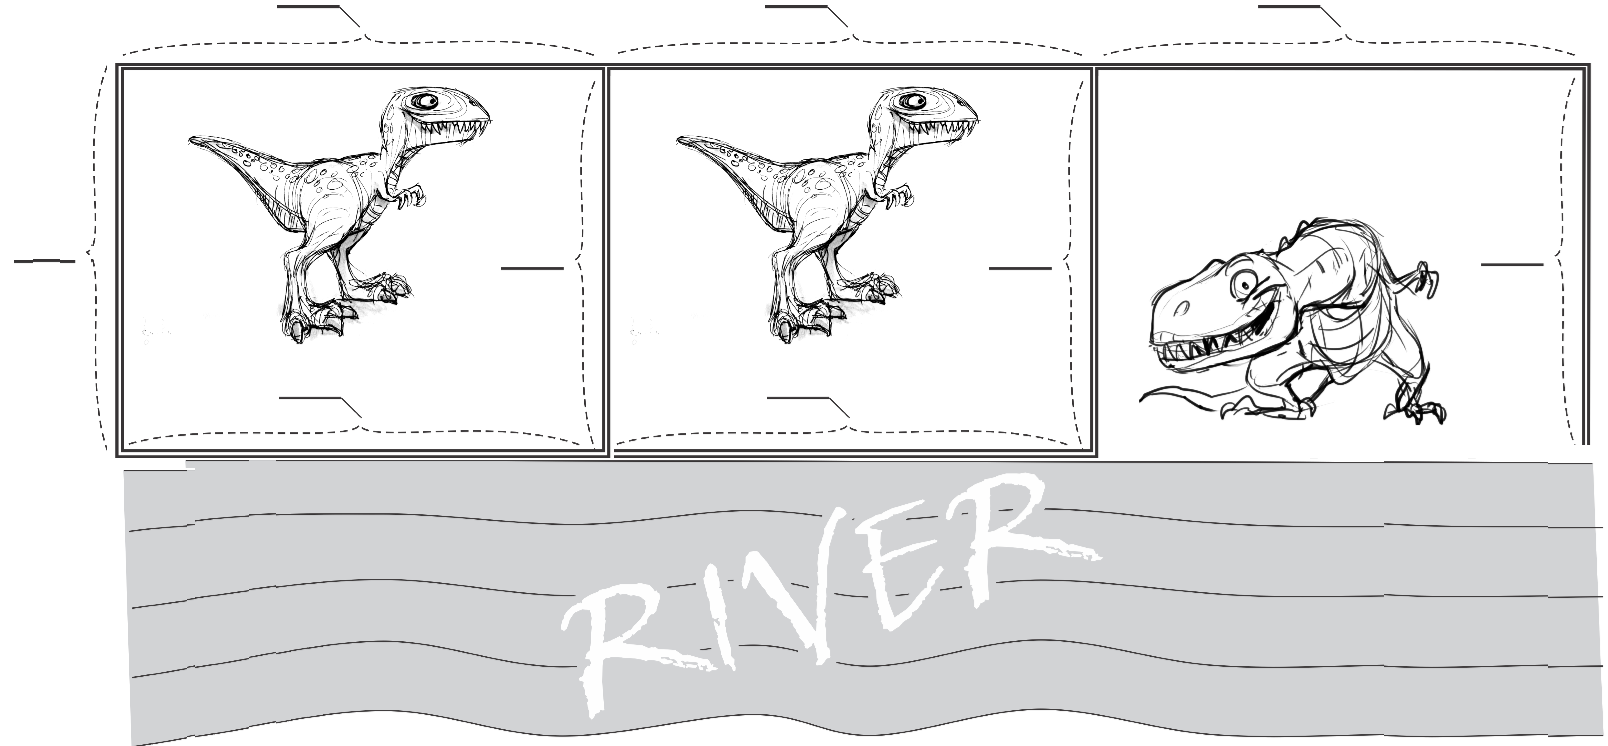
\includegraphics[scale=0.4]{optimization_img_ALT.png}
    \vfill
    \item If you have not completed the Exam prep document, do that now!!
\end{enumerate}




\end{document}
